\section{Finding optimal bandwidth}

\subsection{Part 1}
\subsubsection{(a)}
We are tasked with proving the following equation for the histogram estimator:

\begin{align}
	\int \hat{f}(x)^2 \, dx = \frac{1}{n^2 h} \sum_{j=1}^{m} v_j^2
\end{align}

where \( \hat{f}(x) \) is the histogram estimator, \( v_j \) is the number of
points in the \( j \)-th bin, \( n \) is the total number of points, \( h \) is
the bin width, and \( m \) is the total number of bins.

The histogram estimator \( \hat{f}(x) \) is given by:
\begin{align}
	\hat{f}(x) = \sum_{j=1}^{m} \frac{\hat{p}_j}{h} \mathbb{1}_{[x \in B_j]}
\end{align}
where $\hat{p}_j = \frac{v_j}{n}$ is the estimated probability that a point
falls in the $j$-th bin, and $I_{[x \in B_j]}$ is the indicator
function, which is 1 if $x \in B_j$, and 0 otherwise.

Now, square \( \hat{f}(x) \):
\begin{align}
	\hat{f}(x)^2 = \left( \sum_{j=1}^{m} \frac{\hat{p}_j}{h} \mathbb{1}_{[x \in B_j]} \right)^2
\end{align}
Since the bins \( B_j \) are non-overlapping, the cross terms vanish, and we
are left with:
\begin{align}
	\hat{f}(x)^2 = \sum_{j=1}^{m} \left( \frac{\hat{p}_j}{h} \right)^2 \mathbb{1}_{[x \in B_j]}
\end{align}
Integrating \( \hat{f}(x)^2 \) over the entire domain:
\begin{align}
	\int \hat{f}(x)^2 \, dx = \int \sum_{j=1}^{m} \left( \frac{\hat{p}_j}{h} \right)^2 \mathbb{1}_{[x \in B_j]} \, dx
\end{align}
Because the bins \( B_j \) are disjoint, the integral breaks down into a sum of
integrals over each bin:
\begin{align}
	\int \hat{f}(x)^2 \, dx = \sum_{j=1}^{m} \int_{B_j} \left( \frac{\hat{p}_j}{h} \right)^2 \, dx
\end{align}
The length of each bin is  $h$ and $ \hat{p}_{j}/h $ is independent of x, so
the integral over each bin $B_j$  is:
\begin{align}
	\int_{B_j} 1 \, dx = h
\end{align}
Thus, we get:
\begin{align}
	\int \hat{f}(x)^2 \, dx = \sum_{j=1}^{m} \left( \frac{\hat{p}_j}{h} \right)^2 h = \frac{1}{h} \sum_{j=1}^{m} \hat{p}_j^2
\end{align}
Recall that \( \hat{p}_j = \frac{v_j}{n} \), so we can substitute \( \hat{p}_j^2 \) as:
\begin{align}
	\hat{p}_j^2 = \left( \frac{v_j}{n} \right)^2 = \frac{v_j^2}{n^2}
\end{align}
Thus, the integral becomes:
\begin{align}
	\int \hat{f}(x)^2 \, dx = \frac{1}{h} \sum_{j=1}^{m} \frac{v_j^2}{n^2}
\end{align}
Factor out \( \frac{1}{n^2 h} \):
\begin{align}
	\int \hat{f}(x)^2 \, dx = \frac{1}{n^2 h} \sum_{j=1}^{m} v_j^2
\end{align}
Hence, proved.

\subsubsection{(b)}
Since $\hat{f}_{(-i)}$ is defined as the histogram estimator after removing $i^\text{th}$ observation. 
We have
\begin{align}
	\hat{f}_{(-i)}(X_i) = \sum_{j=1}^{m} \frac{v_j-1}{h(n-1)} \mathbb{1}_{[x \in B_j]}
\end{align}
Since the probability of $x\in B_j$ is $\frac{v_j}{n}$
\begin{align}
	\hat{f}_{(-i)}(X_i)             & = \sum_{j=1}^{m} \frac{v_j}{n} \frac{v_j-1}{h(n-1)}             \\
	\sum_{i=1}^n\hat{f}_{(-i)}(X_i) & =\sum_{i=1}^n \sum_{j=1}^{m} \frac{v_j}{n} \frac{v_j-1}{h(n-1)} \\
	                                & = \frac{1}{(n-1)h}\sum_{j=1}^m (v_j^2 - v_j)
\end{align}

Hence Proved.
\subsection{Part 2}

\begin{enumerate}[label=(\alph*)]
	\item The estimated probabilities for all bins $\hat{p}_j$ is given as:
	      \begin{center}
		      \begin{tabular}{|c|c|}
			      \hline
			      $p_1 = 0.2059$ & $p_2 = 0.4882$    \\ \hline
			      $p_3 = 0.0471$ & $p_4 = 0.0412$    \\\hline
			      $p_5 = 0.1353$ & $p_6 = 0.0588$    \\\hline
			      $p_7 = 0.0059$ & $p_8 = 0.0000$    \\\hline
			      $p_9 = 0.0118$ & $p_{10} = 0.0059$ \\ \hline
		      \end{tabular}
	      \end{center}
	      \begin{figure}[H]
		      \centering
		      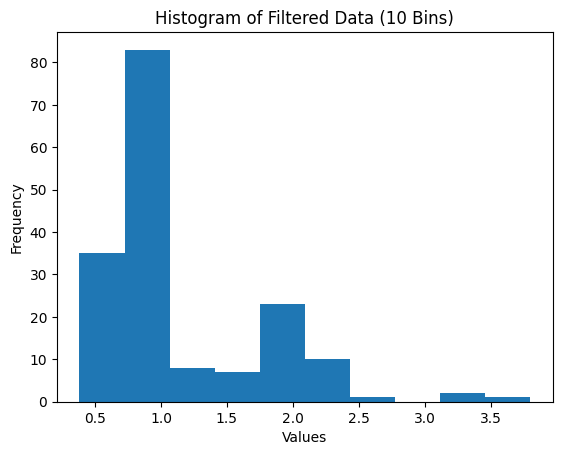
\includegraphics[width=0.7\linewidth]{../images/1/10binhistogram.png}
	      \end{figure}
	\item  The probability distribution is underfit. The binwidth is very large due to which the depiction of data is not quite smooth.
	\item Here's the cross-validation plot:
	      \begin{figure}[H]
		      \centering
		      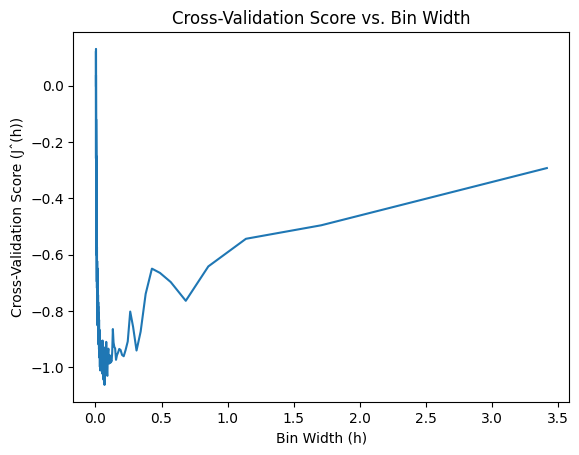
\includegraphics[width=0.7\linewidth]{../images/1/crossvalidation.png}
	      \end{figure}
	\item  The optimal binwidth h is 0.06836.
	\item  The plot seems to give a better analysis of the distribution. It  offers
	      significantly more detail and resolution compared to the 10-bin histogram. Each
	      bin covers a narrower range of data values, leading to a more refined
	      visualization that can better capture small variations in the dataset
	      \begin{figure}[H]
		      \centering
		      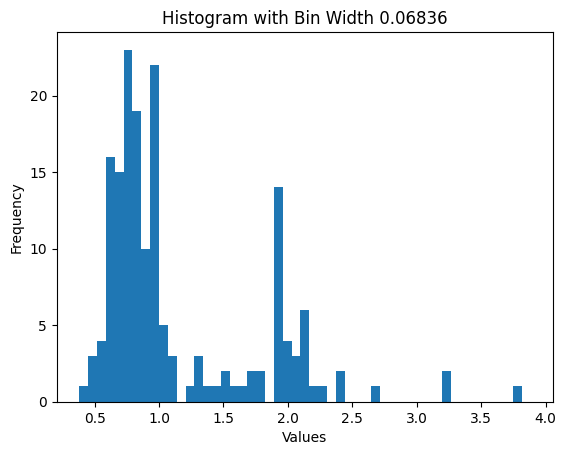
\includegraphics[width=0.7\linewidth]{../images/1/optimalhistogram.png}
	      \end{figure}
\end{enumerate}
